Na literatura, diferentes controladores obtiveram diferentes resultados. 

Em \cite{Boubertakh2013}, foi proposto um controlador PID de atitude cuja resposta é mostrada nas Figuras \ref{fig:Boubertakh2013_pitch} e \ref{fig:Boubertakh2013_roll}. Como se pode ver, a orientação adotada para o ângulo de \textit{pitch}, $\theta$, é invertida em relação à adotada nesse trabalho, mas isso não prejudica a interpretação dos dados. Nota-se que, o sistema para ambos as variáveis convergiu num tempo pouco menor do que dois segundos. O valor exato para o tempo não foi especificado por \citeonline{Boubertakh2013}, mas um valor aproximado pode ser extraído a partir da análise do gráfico.

\begin{figure}[!htb]
    \centering
    \caption{Reposta do ângulo $\theta$ obtido por um controlador PID em \cite{Boubertakh2013}}
    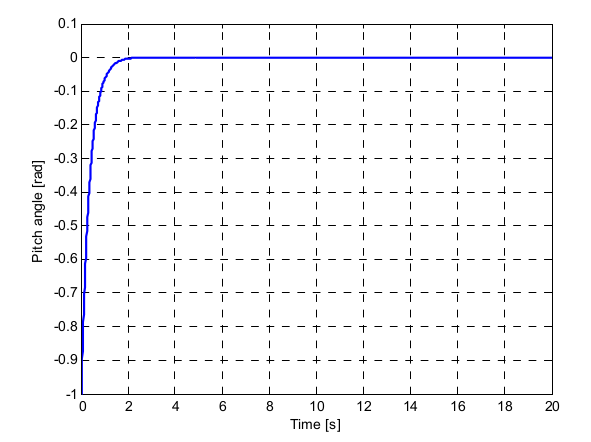
\includegraphics[width=0.6\textwidth]{./04-figuras/resultados/comparacao_outros/18_Boubertakh2013_pitch}
    \fonte{\citeonline{Boubertakh2013}}
    \label{fig:Boubertakh2013_pitch}
\end{figure}
%
\begin{figure}[!htb]
    \centering
    \caption{Reposta do ângulo $\phi$ obtido por um controlador PID em \cite{Boubertakh2013}}
    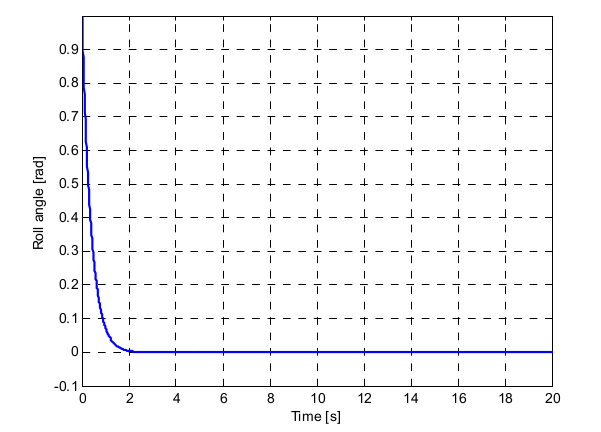
\includegraphics[width=0.6\textwidth]{./04-figuras/resultados/comparacao_outros/18_Boubertakh2013_roll}
    \fonte{\citeonline{Boubertakh2013}}
    \label{fig:Boubertakh2013_roll}
\end{figure}




